\subsection{Anomalous Magnetic Moment of the Muon}
The NP contributions for the anomalous magnetic moment of the muon are described by the parameter set 
\begin{align}
 \left\{m, M_l, g_2^l\right\}.
\end{align}
The Feynman-diagram for this process is depicted in figure \ref{pic_g-2}. 
\begin{figure}[t]
 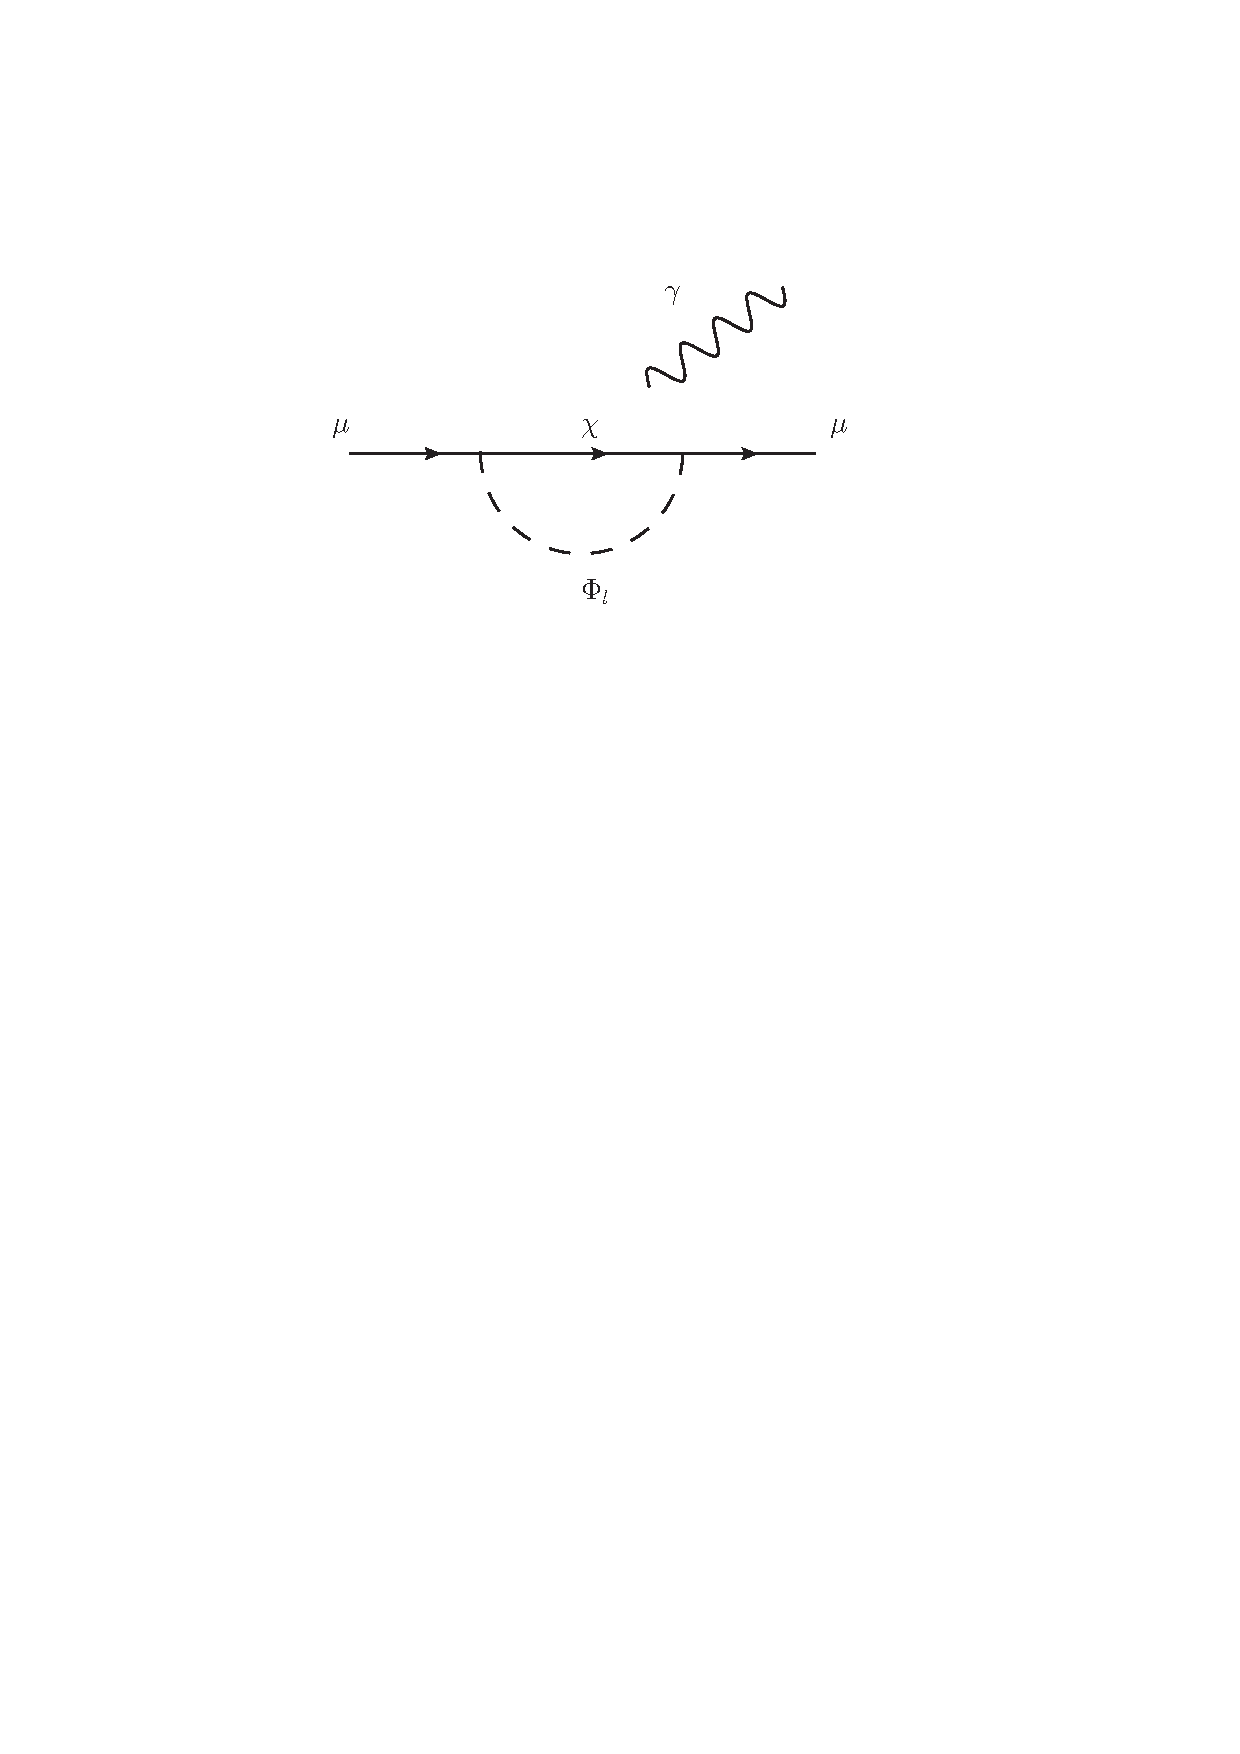
\includegraphics[width=0.6\textwidth]{../pics/g-2.pdf}
 \caption{One-loop contribution to $a_\mu$. Depending on the representations, there are multiple possibilities to attach the photon.}
 \label{pic_g-2}
\end{figure}
Depending on which particle in the loop the photon interacts, there is a different matrix element. If it couples to the scalar, it reads as
\begin{align}
 \mathcal{M}^\rho = |g_2^l|^2 Q_{\Phi_l} e \int\frac{\dx^4 k}{(2\pi)^4} \left[ \frac{2k_\mu k^\rho}{D^\chi_kD^l_{k-p_1}D^l_{k-p_2}} - \frac{k_\mu\left(p_1 +p_2\right)^\rho}{D^\chi_kD^l_{k-p_1}D^l_{k-p_2}} \right] \bar\mu_L(p_2)\gamma^\mu\mu_L(p_1) 
 \label{eq_matg2}
\end{align}
where $Q_{\Phi_l}$ is the electric charge of the boson, $\ti e(2k-p_1-p_2)^\mu$ is the scalar-photon coupling \cite{MDSchwartz}. 
The free Lorentz-index gets contracted with
the polarisation vector $\epsilon_\rho$ of the external photon. With the Gordon identity the vectorial operator is replaced by 
$\sigma^{\mu\nu}q_\nu/2m$ which is necessary to proceed (see sec. \ref{sec_flAnom}). The momentum integral (see \eqref{eq_g2loops})
can be performed \cite{Lavoura} 
where we neglect the external mass and use $q^2=(p_1^2-p_2^2) = 0$ for an on-shell photon. The divergent term from the first term in \eqref{eq_matg2}
cancels out with two-point functions. 
Note that the notation in \cite{Lavoura} is slightly different from ours due to the relative inversion of the squared mass 
fraction $x_l$. 
After gathering everything up and performing the calculation for the fermionic case, we have
\begin{align}
 M^\rho = \frac{|g^l_2|^2}{16\pi^2} \frac{m^2_\mu}{m_\chi^2}\left(Q_\chi^i I(x_l) + Q_{\Phi_l}^i \frac{1}{x_l} I(x_l^{-1}) \right) \bar \mu_L\frac{e\ti\sigma^{\rho\nu}q_\nu}{2m_\mu} \mu_L,
 \label{eq_g-2}
\end{align}
where the sum over $i$ is understood so that for the electric charges, $Q_\mu = Q_\chi - Q_{\Phi_l}$ is ensured and $I$ is a loop function 
(see \eqref{eq_loopmuon}). The NP contribution to $\Delta a_\mu$ can be read off \eqref{eq_g-2}.
